\RequirePackage[l2tabu, orthodox]{nag}

%\documentclass[final, pdftex, a4paper, 12pt, openbib, ]{article}
\documentclass[final, a4paper, openbib, ]{article}
\usepackage[utf8]{inputenc}
\usepackage[french]{babel}
%\usepackage{fontspec}
%\usepackage{lmodern}
\usepackage[T1]{fontenc}
%\usepackage{graphicx}
\usepackage{alltt}
\usepackage{float}
%\usepackage{times}
%\usepackage{a4wide}
\usepackage{upquote,textcomp}
\usepackage{geometry}
%\usepackage{hyperref}
\usepackage{ulem}
\usepackage[
%pdftex,
final,                      % if you do    want to have clickable-colorful links
pdfstartview = FitV,
linktocpage  = false,       % ToC, LoF, LoT place hyperlink on page number, rather than entry text
breaklinks   = true,        % so long urls are correctly broken across lines
pagebackref  = false,     % add page number in bibliography and link to position in document where cited
]{hyperref}
\usepackage{mathtools}
\geometry{a4paper, portrait, margin=2cm}
%\addtolength{\textheight}{2 cm}
%\addtolength{\oddsidemargin}{-1cm}
%\addtolength{\topmargin}{-1cm}
%\addtolength{\textwidth}{1 cm}

%Good solution for monospaces
%\usepackage{pxfonts} % Or palatino or mathpazo, changes all fonts to something sans
%\usepackage{eulervm} % only changes math fonts, i checked
%\usepackage[ttdefault=true]{AnonymousPro} %Only changes tt fonts
% WHICH ONE TO CHOOSE?
%\usepackage{pslatex}
%\usepackage[ttdefault=true]{AnonymousPro} %Only changes tt fonts
% \usepackage[varg, cmintegrals, cmbraces, ]{newtxtext,newtxmath} % libertine, uprightGreek (U.S.) or slantedGreek (ISO), 
% \usepackage{tgtermes}
% \usepackage{txfonts}
% \usepackage{mathptmx}
% \usepackage[scaled=.90]{helvet}
% \usepackage{courier}
% \usepackage{textcomp}     % required for special glyphs
% \usepackage{bm}   


\usepackage{caption}
\captionsetup[figure]{labelformat=empty}% redefines the caption setup of the figures environment in the beamer class.

%Inconsoloata, a little too light.
%\usepackage{inconsolata}
%\renewcommand{\ttdefault}{Consolas}
%\usepackage{fontspec} %Doesn't work with pdflatex
%\setmonofont{Consolas}

%\renewcommand*\familydefault{\ttdefault} %% Only if the base font of the document is to be typewriter style
%\newcommand\Fontvi{\fontsize{6}{7.2}\selectfont}

%Make tabularx center cells vertically
%\def\tabularxcolumn#1{m{#1}}
%\renewcommand{\tabularxcolumn}[1]{>{\small}m{#1}}

%%Syntax hilighting
%\usepackage{fancyvrb}
\usepackage{minted}
%\usepackage[newfloat]{minted}
\usemintedstyle{borland}
%\usepackage{etoolbox}
%\AtBeginEnvironment{minted}{\singlespacing%
%	\fontsize{14}{14}\selectfont}
%\newminted{java}{fontsize=\footnotesize}
\usepackage{caption}

%\usepackage{multicol}
%\usepackage{vwcol}
%\usepackage{lipsum}
%\usepackage{microtype}
%\setlength{\columnseprule}{0.4pt}
%\renewcommand{\columnseprulecolor}{\color{red}}
\newcommand{\BAD}[1]{{\color{red}#1}}
\newcommand{\GOOD}[1]{{\color{darkgreen}#1}}


\usepackage{graphicx}
\usepackage{colortbl,array}
\usepackage{tabularx}
\definecolor{warningbackground}{RGB}{252,226,158}

\newcommand{\alertwarningbox}[1]{
	\centering
	\begin{tabularx}{0.9\linewidth}{
			>{\columncolor{warningbackground}}c
			>{\columncolor{warningbackground}}X}
		\raisebox{\dimexpr2\baselineskip-\height}
		{
\includegraphics[scale=0.8]{\images/Information.pdf}}&
		\raisebox{\tabcolsep}{\strut}#1\raisebox{-\tabcolsep}{\strut}
	\end{tabularx}
}


\usepackage{xcolor}

%\definecolor{infobackground}{RGB}{217,237,247}
%\definecolor{infoforeground}{RGB}{58,135,173}
%\definecolor{infoborder}{RGB}{188,232,241}

\definecolor{infobackground}{RGB}{217,237,247}
\definecolor{infofrancaisforeground}{RGB}{30,50,70}
\definecolor{infoborder}{RGB}{30,50,70}

\definecolor{infobackground}{RGB}{217,237,247}
\definecolor{infoforeground}{RGB}{30, 80, 150}
\definecolor{infoborder}{RGB}{47, 87, 232}

% ORANGE
\definecolor{infobackground2}{RGB}{255,210,180}
\definecolor{infoforeground2}{RGB}{212, 50, 0}
\definecolor{infoborder2}{RGB}{255, 90, 20}

% GREEN
\definecolor{infobackground3}{RGB}{223,251,223}
\definecolor{infoforeground3}{RGB}{25, 150, 25}
\definecolor{infoborder3}{RGB}{55, 220, 55}


\usepackage{environ}
\usepackage{tikz}
\usetikzlibrary{fit,backgrounds,calc}

\NewEnviron{alertinfo}[1]
{
	\begin{center}
		\begin{tikzpicture}
		\node[inner sep=0pt,
		draw=infoborder,
		line width=1pt,
		fill=infobackground] (box) {\parbox[t]{0.99\textwidth}
			{%
				\begin{minipage}{.12\textwidth}
				\centering\tikz[scale=3]
				\node[scale=1]
				{
					
\includegraphics[scale=0.25]{\images/Information.pdf}
				};
				\end{minipage}%
				\begin{minipage}{.86\textwidth}
				\vskip 10pt
				\textbf{\textcolor{infoforeground}{\large #1}}\par\smallskip
				\textcolor{infoforeground}{\large \BODY}
				\par\smallskip
				\par\smallskip
				\end{minipage}\hfill
			}%
		};
		\end{tikzpicture}
	\end{center}
}


\NewEnviron{alertinfo2}[1]
{
\begin{center}
    \begin{tikzpicture}
    \node[inner sep=0pt,
          draw=infoborder2,
          line width=1pt,
          fill=infobackground2] (box) {\parbox[t]{0.99\textwidth}
        {%
            \begin{minipage}{.12\textwidth}
                \centering\tikz[scale=3]
                \node[scale=1]
                {
                    
\includegraphics[scale=0.25]{\images/Information_orange.pdf}
                };
            \end{minipage}%
           \begin{minipage}{.86\textwidth}
                \vskip 10pt
                \textbf{\textcolor{infoforeground2}{\large #1}}\par\smallskip
                \textcolor{infoforeground2}{\large \BODY}
                \par\smallskip
                \par\smallskip
            \end{minipage}\hfill
        }%
    };
    \end{tikzpicture}
\end{center}
}


\NewEnviron{alertinfo3}[1]
{
\begin{center}
    \begin{tikzpicture}
    \node[inner sep=0pt,
          draw=infoborder3,
          line width=1pt,
          fill=infobackground3] (box) {\parbox[t]{0.99\textwidth}
        {%
            \begin{minipage}{.12\textwidth}
                \centering\tikz[scale=3]
                \node[scale=1]
                {
                    
\includegraphics[scale=0.25]{\images/Information_green.pdf}
                };
            \end{minipage}%
           \begin{minipage}{.86\textwidth}
                \vskip 10pt
                \textbf{\textcolor{infoforeground3}{\large #1}}\par\smallskip
                \textcolor{infoforeground3}{\large \BODY}
                \par\smallskip
                \par\smallskip
            \end{minipage}\hfill
        }%
    };
    \end{tikzpicture}
\end{center}
}

\usepackage{titling}

\newif\ifDRAFT
\DRAFTtrue
% Only comment and uncomment false line :
%\DRAFTfalse

\ifDRAFT
	%Hilighting commands:
	\newcommand{\hl}[1]{\textcolor{green}{#1}}
	\newcommand{\fix}[1]{\textcolor{red}{#1}}	
	\newcommand{\todo}[1]{{\color{red}\bf\em TODO:\/\@#1}}
%	\newcommand{\todo}[1]{{}}	
	\newcommand{\comment}[1]{{\color{blue}\bf\em Comment: \/\@#1}}
%	\newcommand{\comment}[1]{{}}	
	
	\newcommand{\hll}[1]{\textcolor{orange}{\sout{#1}}}
	%\newcommand{\hll}[1]{{}}
	\newcommand{\WR}[1]{\textcolor{purple}{#1}}
\else
	% for final sub
	\newcommand{\hl}[1]{#1}	
	%\newcommand{\hl}[1]{\textcolor{dkgreen}{#1}}
	\newcommand{\fix}[1]{{}}
%	\newcommand{\fix}[1]{\textcolor{red}{#1}}
	\newcommand{\todo}[1]{{}}
	\newcommand{\hll}[1]{{}}
	\newcommand{\comment}[1]{{}}
	\newcommand{\WR}[1]{{#1}}
%	\newcommand{\WR}[1]{\textcolor{purple}{#1}}	
\fi


\newcommand{\codes}{codes}
\newcommand{\images}{images}

%FIX FOR : Undefined control sequence. \tightlist
\providecommand{\tightlist}{%
  \setlength{\itemsep}{0pt}\setlength{\parskip}{0pt}}
  

%\title{GBIAAL 4$^{\mbox{\`eme}}$ année \\ Devoir Surveillé --- Base de données \\ 13 janvier 2016  \\ 1 heure}
\title{GIS 3$^{\mbox{\`eme}}$ année
	%\\TP1 Structures, Listes contiguës, Redirections}
}
\author{\huge \textbf{Introduction à} \\  \Huge\textbf{\texttt{git}}}
\setlength{\parindent}{0pt}
%\pagestyle{empty}
\date{\Large \url{https://rudametw.github.io/teaching/} \\ Polytech Lille}

%\author{Walter Rudametkin}
%\institute[Polytech Lille]{
%Walter.Rudametkin@polytech-lille.fr\\
%\url{https://rudametw.github.io/teaching/}\\
%\vspace{0.5cm}Bureau F011\\
%Polytech Lille\\

\begin{document}
%\vspace{-15cm}
\vspace{-4.5cm}
\posttitle{\par\end{center}}
\setlength{\droptitle}{-45pt}
\maketitle
%\thispagestyle{empty}

\section{Objectifs}\label{objectifs}

\begin{itemize}
\item Apprendre à se servir d'un Logiciel de Gestion de Version.
\item Maitrisez le versionnement d'un projet logiciel.
\item Partager un projet et travailler en équipe.
\end{itemize}

\begin{alertinfo}{IMPORTANT !}
Lisez attentivement la sortie de \textbf{\textit{chaque}} commande \texttt{git}.
Il est fortement conseiller de travailler exclusivement sur terminal pour ce TP.
%Nous vous proposerons régulièrement d'exécuter des commandes dans un terminal 
\end{alertinfo}

%\paragraph{Contexte et préparation : } 
\section{Contexte et préparation } 

\subsection{Configuration de \texttt{bash}}

\paragraph{\texttt{.bashrc} et \texttt{gitprompt.sh}}
Pour commencer ce TP, nous vous fournissons une configuration plus avancé pour \texttt{bash} (l'interpréteur en ligne de commande utilisé par défaut).
Vous pouvez lancer, une seule fois par compte, la commande suivante qui aura pour objectif de mettre à jour votre fichier \texttt{~/.bashrc} et d'installer \texttt{gitprompt.sh} sur vos comptes.
\begin{minted}[mathescape=true,escapeinside=||,tabsize=4
%	,fontsize=\footnotesize,
]{bash}
	~wrudamet/public/set_bashrc.sh
\end{minted}

Pour les curieux, vous pouvez regarder vos fichiers \mintinline{bash}{~/.bashrc}, \mintinline{bash}{~/.bashrc-students} et \mintinline{bash}{~/git-prompt.sh} pour comprendre ce qui a été ajouté.


\paragraph{Terminals}
%\WR{Copier le fichier XXX.aide pour récupèrer quelques commandes. }
Nous vous proposons de travailler sur plusieurs terminals ouverts simultanément, une disposition possible est indiqué dans la figure~\ref{terminals} mais vous pouvez les ranger à votre convenance tout au longue du TP.
\begin{figure}[h]
	\centering
	{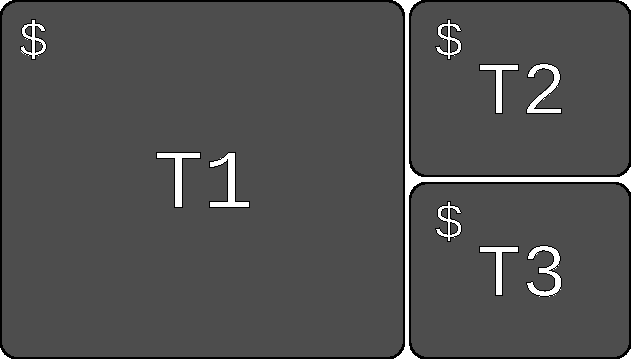
\includegraphics[scale=0.5]{images/terminals.pdf}}
	\caption{Figure 1: Disposition des terminals proposée.}
	\label{terminals}
\end{figure}

Cette disposition vous permettra d'exécuter vos commandes \texttt{git} dans le terminal \texttt{T1}, tout en vous permettant d'exécuter des commandes de suivi dans les terminaux \texttt{T2} et \texttt{T3}.~\ref{terminals}\\

Dans un premier temps, positionnez \texttt{T1}, \texttt{T2} et \texttt{T3} dans le répertoire où vous allez travailler.\\

Ensuite, dans le terminal \texttt{T2} exécutez :
\begin{minted}[mathescape=true,escapeinside=||,tabsize=4
%	,fontsize=\footnotesize,
]{bash}
	watch -d -n3  'tree -a tpgit'
\end{minted}

Ensuite, dans le terminal \texttt{T3} exécutez :
\begin{minted}[mathescape=true,escapeinside=||,tabsize=4
%	,fontsize=\footnotesize,
]{bash}
	watch 'cat .gitconfig'
\end{minted}

C'est normal que ces commandes affichent des erreurs car nous n'avons pas encore crée le répertoire \texttt{tpgit} ni le fichier \texttt{.gitconfig}.


\subsection{Configuration de votre compte \texttt{git}}

Il est important de savoir qui a fait quoi. \texttt{git} a besoin d'une configuration pour identifier vos futurs commits, et vous pouvez également spécifier certaines comportements.
Les commandes suivantes vont modifier votre fichier \texttt{.gitconfig}, tapez les en regardent les changements dans le terminal \texttt{T3}:

\begin{minted}[mathescape=true,escapeinside=||,tabsize=4
%	,fontsize=\footnotesize,
]{bash}
	git config --global user.name "votre nom"
	git config --global user.email nom.prenom@polytech-lille.net
	git config --global core.editor kate
	git config --global push.default simple
\end{minted}

Si vous préférez un autre éditeur, vous pouvez l'utiliser à la place de \texttt{kate}.

\begin{alertinfo}{Attention !}
La configuration de \texttt{git} et de \texttt{bash} doit se faire une fois pour chaque compte.
Votre binôme devra réaliser la même configuration sur son compte, et si vous comptez travailler sur un autre PC, il faudra récupérer votre fichier \texttt{.gitconfig} ou relancer les commandes de configuration.
\end{alertinfo}

\section{Initialisation d'un dépôt \texttt{git}}

Nous allons travailler sur un projet qu'on appellera \texttt{tpgit}. En vous aidant des supports du cours (slide 13), vous devez :
\begin{itemize}
\item créer un répertoire \texttt{tpgit}
\item initialiser dans ce répertoire, un dépôt git vide
\item regarder les fichiers crées pour ce dépôt, elles seront affichés dans le terminal \texttt{T2}
\item créer un fichier \texttt{fruits.txt}
\item réaliser un commit en ajoutant 2 fruits à \texttt{fruits.txt}. Pour rappel, l'enchainement des commandes est : \mintinline{bash}{status, add, status, commit, status, log}.
Lisez la sortie de chaque commande pour comprendre leur fonctionnement.
\item réaliser 3 commits de plus en ajoutant à chaque fois des fruits.
\end{itemize}

\begin{alertinfo3}{Astuce !}
Utilisez les commandes \texttt{git status}, \texttt{git diff \textit{nom\_fichier}} et \texttt{git log} pour comprendre l'état de votre dépôt. La commande \texttt{git log -}\texttt{-graph -}\texttt{-oneline -}\texttt{-decorate -}\texttt{-all} vous donne une historique détaillé avec toutes les branches, étiquettes et commits.
Pour quoi ne pas la garder à la vu dans le terminal \texttt{T3} (l'éxécuter avec un \texttt{watch -d -n5 git log \ldots}) ?
\end{alertinfo3}


\section{Branches \texttt{git}}

Branches \texttt{legumes}
\begin{itemize}
\item créer une branche \texttt{legumes}
\item ajouter un fichier \texttt{legumes.txt} sur cette branche
\item réaliser 3 commits différents en ajoutant des légumes à \texttt{legumes.txt}
\item vérifier l'historique de vos commits à l'aide de \texttt{git log}.
\end{itemize}

Branches \texttt{sauces}
\begin{itemize}
\item créer une branche \texttt{sauces}
\item ajouter un fichier \texttt{sauces.txt} sur cette branche
\item réaliser 2 commits différents
\item vérifier l'historique de vos commits et l'existence de \textbf{3 branches} (master, legumes, sauces) à l'aide de \texttt{git log}.
\end{itemize}

\section{Merges \texttt{git}}
Vous avez décidé que vos commits dans les branches \texttt{legumes} et \texttt{sauces} sont pertinents, maintenant vous devez les intégrer dans \texttt{master}.
\begin{itemize}
\item allez sur la branche legumes
\item vérifier l'état de votre espace de travail (e.g., l'inéxistance du fichier \texttt{sauces.txt})
\item merger \texttt{master} dans \texttt{legumes}
\item si tout va bien, mergez \texttt{legumes} dans \texttt{master}
\item vérifier l'historique de vos commits et l'apparition de \texttt{legumes.txt} sur la branche \texttt{master}\\
\end{itemize}

Vous pouvez maintenant merger la branche \texttt{sauces} avec \texttt{master}.

\section{Dépôt distant}

Nous allons activer vos comptes sur le serveur GitLab de Polytech et créer un dépôt vide où vous allez pousser votre dépôt existant \texttt{tpgit}.
GitLab vous permet de gérer votre projet et fourni plusieurs fonctionnalités intéressantes (e.g., issues, graphes, édition de fichiers).\\

Vous devez :
\begin{itemize}
\item Vous connectez sur \url{https://archives.plil.fr/}
\item Créer un projet sur le serveur GitLab de Polytech
\item Pousser votre dépôt \texttt{tpgit} sur le GitLab
\item Ajouter votre binôme aux membres de votre projet avec le niveau de droit Developer (il devra se connecter une première fois avant d'apparaitre dans la liste de membres)
\end{itemize}

\paragraph{Créer un dépôt sur GitLab et poussez \texttt{tpgit}}
\begin{enumerate}
\item Cliquer sur \textit{+New Projet} en haut pour créer un nouveau projet
\item Donner un nom à votre projet et cliquer sur \textit{Create project}
\item Vous êtes emmenés dans votre projet, qui est vide, avec les instructions des différentes formes d'initialisation.
Lisez les propositions.
Vous devez \textbf{impérativement changer l'url de \texttt{SSH} à \texttt{HTTPS}}
\item Retrouvez les instructions \textit{Push an existing Git repository}. Vous allez copier et exécuter la commande :\\ \texttt{git remote add origin https://archives.plil.fr/<user>/<project.git>} avec le bon url\\ suivi de \texttt{git remote -v}, et \texttt{git push -u origin master}
\item Rafraichissez la page de votre projet GitLab, votre projet \texttt{tpgit} doit s'y retrouver
\item Naviguez votre projet pour voir l'historique de commits (\textit{Files, Commits, Network}).
\end{enumerate}

\begin{alertinfo2}{Attention !}
Il y a deux protocoles réseau pour intéragir avec GitLab, HTTPS et SSH. Nous vous conseillons de travailler avec HTTPS dans un premier temps.
Dans le futur vous pouvez choisir SSH mais il faudra configurer vos clés privés et publiques en suivant l'aide \url{https://archives.plil.fr/help/ssh/README}
\end{alertinfo2}


\paragraph{Gestion des membres de votre projet}
\begin{enumerate}
\item Aller dans les Settings de votre projet (menu à gauche),
\item Cliquer sur Members dans le menu Settings (menu à gauche),
\item Cliquer sur New project member en haut à droite,
\item Chercher le login de la personne que vous voulez ajouter,
\item Sélectionner le niveau de droit de cette personne,
\item Cliquer sur Add users.
\end{enumerate}



\pagebreak

\begin{alertinfo}{Attention !}
\end{alertinfo}
\begin{alertinfo2}{Attention !}
\end{alertinfo2}
\begin{alertinfo3}{Astuce !}
\end{alertinfo3}






\subsection{Chargement à partir d'un fichier}


\begin{enumerate}
\item 
\item 
\end{enumerate}

\section{Questions s’il vous reste du temps}

\pagebreak

\section{Annexes}
\vspace{-0.5cm}
\begin{figure}[!h]
	\begin{minipage}[c]{0.40\textwidth}
		\centering
		\inputminted[
		%frame=lines,
		%framesep=2.5mm,
		%baselinestretch=0.8,
		fontsize=\small,
		linenos,
		tabsize=2,
		breaklines,
		xleftmargin=-25pt,
		numbersep=7pt,		
		%firstline=14,lastline=28
		%bgcolor=light-gray
		]
		{c}{\codes/ldc.c}
		\caption{\texttt{ldc.c}}
	\end{minipage}
	\hspace{0.1cm}
	\vrule{}
	\hspace{0.3cm}
	\begin{minipage}[c]{0.62\textwidth}
		%		\centering
		\inputminted[
		%frame=lines,
		%framesep=2.5mm,
		%baselinestretch=0.8,
		fontsize=\small,
		linenos,
		tabsize=4,
		breaklines,
		xleftmargin=4pt,
		numbersep=7pt,
		%		breaksymbolleft=,
		%firstline=14,lastline=28
		%bgcolor=light-gray
		]
		{c}{\codes/moyenne_fichier.c}
		\centering
		%		\captionof{listing}{entiers.txt}
		%		\captionsetup[justification=justified,singlelinecheck=false]
		%		\captionsetup{justification=raggedright, singlelinecheck=false}
		\caption{\texttt{moyenne\_fichier.c}}
	\end{minipage}
	%	\hspace{-1cm}
	%	\vrule{}
	%	\hspace{0.6cm}
	%	\begin{minipage}[b]{0.15\textwidth}
	%		\centering
	%		\inputminted[
	%		%frame=lines,
	%		%framesep=2.5mm,
	%		%baselinestretch=0.8,
	%		fontsize=\small,
	%		linenos,
	%		tabsize=2,
	%		%firstline=14,lastline=28
	%		%bgcolor=light-gray
	%		]
	%		{c}{\codes/moyenne_fichier.c}
	%		\captionsetup{justification=raggedright, singlelinecheck=false}
	%		\caption{annu.txt}
	%	\end{minipage}
	%	\captionof{listing}{SomeCaption}
	%	\label{lst:representation_examples}
\end{figure}
\end{document}